%------------------------------------------------------------------------------
% Template file for the submission of papers to IUCr journals in LaTeX2e
% using the iucr document class
% Copyright 1999-2013 International Union of Crystallography
% Version 1.6 (28 March 2013)
%------------------------------------------------------------------------------

\documentclass[preprint]{iucr}              % DO NOT DELETE THIS LINE

     %-------------------------------------------------------------------------
     % Information about journal to which submitted
     %-------------------------------------------------------------------------
     \journalcode{S}              % Indicate the journal to which submitted
                                  %   A - Acta Crystallographica Section A
                                  %   B - Acta Crystallographica Section B
                                  %   C - Acta Crystallographica Section C
                                  %   D - Acta Crystallographica Section D
                                  %   E - Acta Crystallographica Section E
                                  %   F - Acta Crystallographica Section F
                                  %   J - Journal of Applied Crystallography
                                  %   M - IUCrJ
                                  %   S - Journal of Synchrotron Radiation

\begin{document}                  % DO NOT DELETE THIS LINE

     %-------------------------------------------------------------------------
     % The introductory (header) part of the paper
     %-------------------------------------------------------------------------

     % The title of the paper. Use \shorttitle to indicate an abbreviated title
     % for use in running heads (you will need to uncomment it).

\title{New data analysis pipeline for the BioSAXS beamline at the ESRF}
%\shorttitle{Short Title}

     % Authors' names and addresses. Use \cauthor for the main (contact) author.
     % Use \author for all other authors. Use \aff for authors' affiliations.
     % Use lower-case letters in square brackets to link authors to their
     % affiliations; if there is only one affiliation address, remove the [a].

\cauthor[a]{Jérôme}{Kieffer}{jerome.kieffer@esrf.fr}
\author[a]{Martha}{Brennich}
\author[b]{Jean-Baptiste}{Florial}
\author[a]{Marcus}{Oscarson}
\author[a]{Alejandro}{De Maria Antolinos}
\author[a]{Mark}{Tully}
\author[a]{Petra}{Pernot}
\aff[a]{The European Synchrotron, 71 Avenue des Martyrs, 38000 Grenoble \country{France}}
\aff[b]{European Molecular Biology Laboratory, 71 Avenue des Martyrs, 38000 Grenoble \country{France}}


     % Use \shortauthor to indicate an abbreviated author list for use in
     % running heads (you will need to uncomment it).

\shortauthor{Kieffer and Brennich}

     % Use \vita if required to give biographical details (for authors of
     % invited review papers only). Uncomment it.

%\vita{Author's biography}

     % Keywords (required for Journal of Synchrotron Radiation only)
     % Use the \keyword macro for each word or phrase, e.g. 
     % \keyword{X-ray diffraction}\keyword{muscle}

\keyword{online data analysis; solution scattering; proteins; biological small-angle X-ray scattering; 
automation; high brilliance; structural biology;
BioSAXS; high-throughput SAXS;  size-exclusion chromatography; online purification}

     % PDB and NDB reference codes for structures referenced in the article and
     % deposited with the Protein Data Bank and Nucleic Acids Database (Acta
     % Crystallographica Section D). Repeat for each separate structure e.g
     % \PDBref[dethiobiotin synthetase]{1byi} \NDBref[d(G$_4$CGC$_4$)]{ad0002}

%\PDBref[optional name]{refcode}
%\NDBref[optional name]{refcode}

\maketitle                        % DO NOT DELETE THIS LINE

\begin{synopsis}
Detailed presentation of the automatic data analysis pipelines for the BioSAXS beam-line at the European synchrotron.  
\end{synopsis}

\begin{abstract}
context
purpose
method
major results
major conclusions

Abstract goes here.
\end{abstract}


     %-------------------------------------------------------------------------
     % The main body of the paper
     %-------------------------------------------------------------------------
     % Now enter the text of the document in multiple \section's, \subsection's
     % and \subsubsection's as required.

\section{Introduction}
Small angle scattering (SAS) provides low resolution information on macromolecules and it is  
particularly suited for biological sample thanks to the absence of lengthy preparation. 
Biologists expects from SAXS experiment to retrieve the size and the shape of their protein or complex under study.
Automated analysis is hence of crucial importance for them.

The BioSAXS \cite{BM29paper} beamline had an automated pipeline for the data-analysis which was based on EDNA\cite{EDNA} and the ATSAS\cite{ATSAS2}
software. 
While the outcome of the processing was very appreciated by our users, the system was already close to the maximal throughput possible in terms of performances. 
The new EBS source \cite{EBS} of the ESRF not only provides a higher brilliance, but also new wiggler sources for former bending-magnet beamlines which triggered the re-build and the upgrade of most of them. 
Thus the BioSAXS beamline has been rebuilt and features a new flight-tube with its Pilatus 2M detector mounted in vaccum. 

This contribution is divided in two main parts, starting with presentation of the tools used for 
processing SAS data (\textit{FreeSAS}) and for assembling pipelines (\textit{Dahu}).
Then the different pipelines are presented, the common for the reduction of the scattering images and two dedicated for sample-changer and SEC-SAXS experiments.      

\section{Tools}

To reach the 10-fold speed up expected from the new EBS source and the new detector (Upgrade from a Pilatus 1M to a 2M with a thick sensor, mounted \textit{in vacuum})
all software used at the beamline was upgraded.
Precise benchmarking of the execution times of the previous EDNA-based pipeline demonstated that 
most time was spent in launching external tools coming from the ATSAS suite and in parsing text files produced by those tools.
It was descided to rewrite all pipeline in plain Python \cite{python} and call SAS-related tasks from a library, \textit{FreeSAS}. 
Finally the interface to the control software, Bliss \cite{bliss}, would go via Tango \cite{tango} and use a simple FIFO task scheduler,  \textit{dahu}, 
already used in production on another SAXS beamline at the ESRF: ID02\cite{ID02}.   

\subsection{The SAS processing tools, \textit{FreeSAS}}

\textit{FreeSAS} is a Python\cite{python} library containing SAS analysis tools available both via command like interface and from the Python API. 
It does not claim to be as complete as the ATSAS counterpart,
but is free, released under the MIT license (i.e. it can be included in commercial products), all source code is available publicly on github \cite{freesas} and
open to contributions.
Despite Python being an interpreted language, FreeSAS is performance oriented and most of the processing is performed in Cython\cite{cython} extensions written in C 
to obtain the seeked performances. 
All the code has been made available and packaged independently from the online analysis tools to offer ESRF users and other scientists
the ability to reprocess their data and compare the processing between software and sources.

\subsubsection{SAS plotting}

TODO: insert an image  of the tool
Note:
$q = 4\pi sin(2\theta/2)$

\subsubsection{Guinier region fitting}
Guinier analysis \cite{guinier} is usually the first analysis performed in BioSAXS to determine the radius of gyration ($R_g$)of the macromolecule (and the forwards scattering value $I_0$.
$R_g$ is obtained from the slope of a linear regression of $ln(I)$ as function of $q^2$ on the proper q-range where this curve is afine (the Guinier-range).
The selection of the Guinier-range is far from being obvious since most of subsequent analysis depend on the proper assesement of this regions, 
multiple implementation are provided: \textit{autorg.py} which derives from the BioXTAS-RAW\cite{bioxtasraw}, \textit{auto_guinier.py} which differs from the BioXTAS-RAW
one by searching for a consensus region rather than the best region. 
\textit{auto_gpa.py} performs a Guinier-peak-analysis\cite{gpa}, which is a quick assessment of the $R_g$ and $I_0$ and sometimes less robust than the two other implementations. 

It is worth mentionning that none of the three algorithms are provided the exact same results as the AUTORG\cite{ATSAS2} version from ATSAS. 
This highlights the importance of publishing the actual implementation of the algorithms with the associated numerical constants.
  
\subsubsection{Pair distribution function}
Despite the scattering curve ($I(q)$) is the Fourier transform of the pair distribution function $p(r)$, the later cannot directly be obtained from the
inverse Fourier tranform (IFT due to the loss of phase information and the limited amount of information in the scattering curve. 
This ill-posed mathematical has not exact solution and is usually inversed with some extra constraints imposed, like the finite size of the support (defined by the maximum diameter, $Dmax$).    
FreeSAS proposes an IFT based on the Bayesian statistics and derived from BIFT\cite{bift}, like the one found in \cite{bioxtasraw}.
The command-line programme to perfrom and IFT is \textit{bift.py}. 
Despite the approach differs, the results of \textit{bift.py} is similar to the DATGNOM\cite{ATSAS1} from ATSAS which uses a Tikhonov's regularization.
The diameter found, $Dmax$, is directly comparable with the one provided by ATSAS, but the parameter $\alpha$ differs since the theory used for the regularisation differs. 

\subsubsection{Equivalence of scattering curves}
To obtains the best possible signal from the sample, the capillary is exposed multiple times with a short exposure time.
All equivalent frames are then merged to optimized the signal/noise ratio without polluting the signal with radiation damage.  
The equivalence of frames is obtained from the \textit{CorMap} \cite{cormap} implementated from the publication. 

\subsubsection{Overlay of bead models}
FreeSAS features also \textit{subpycomp} \cite{BM29ODA}, a tool to rotate/flip bead models and overlay them prior to merge them. It is equivalent to the SUPCOMB\cite{supcomb} tool from ATSAS. 

\subsection{The workflow manager: \textit{dahu}}

The role of the workflow manager is to ensure all the processing requested by the user interface is actually performed and that the client is warned in case of issue.
This subsection is purely technical and can be skipped. 

EDNA\cite{EDNA} was used as workflow manager for the previous data-analysis pipeline for many protein crystallography beamlines and the BioSAXS beamline at the ESRF \cite{BM29ODA}.
The parallelization model implemented in EDNA is based on Python threads and forking processes. 
Despite the Global Interpreter Lock (GIL) which prevents Python from running multiple threads simultaneously, parallel processing occues when the work is performed
in separated process. 
This implies that for each task to be perfomed, an input file needs to be written before launching the process and the result file needs to be read and parsed after the end of the processing.
When processing was doing loops of jobs, most of the time was spent in string manipulation for writing and parsing strings (for example: to compare pair-wise 10 frames it takes 45 process to be launched !)
 
The \textit{dahu} workflow manager was designed for the TruSAXS beamline \cite{ID02} with those limitation in mind. 
Text manipulation was simplfied by switching from XML to JSON data-structure representation. 
This modification alone has proven to speed up EDNA by a factor 3 !

Most of the idea implemented in the EDNA framework were keps and the code was simplified to the extreme since \textit{dahu} represents only 1000 lines of code. 
The scheduling of jobs is performed via a shared queue (hence First-in-First-out) and only a limited number of them are allowed to run simultaneously, via theads.
The parallelization can only occure only in sections of code which release the GIL, this is why FreeSAS is mostly implemented in Cython (and GIL-free).      

\subsubsection{Jobs}

The \textit{dahu-job} is the interface with the outer world. 
It manages the execution identifier, exposes the status and controls the execution workflow of the underlying plugin via the \textit{setup-process-teardown} sequence.
Unlike EDNA, in \textit{dahu}, only jobs see their input and output saved to the disk to allow off-line reprocessing.   

\subsubsections{Plugins}
Plugins are Python \textit{function} or \textit{classes} which are provided externally (by the beamlinee scientist) and implement the actual processing.
The plugins are fairly independent of the \textit{dahu} framework and hence rather easy to implement in pure Python.
For example the three plugins described in section \ref{pipeline} account each for about 700 lines of code.  

\subsubsection{Online processing}
Online processing is achieved by exposing \textit{dahu-jobs} via a Tango interface.

\subsubsection{Offline processing}
Dahu provides also a command-line tool, called \textit{dahu-reprocess} designed to (re-)execute one or several pipelines based on the job-description saved. 
This tool is also used for testing pipelines offline.
Dahu has virtually no dependencies (beside Python) and can deployed on any computer to reprocess complete datasets. 
To reprocess data acquired at the BioSAXS beamline from ESRF, one would of course need FreeSAS and other dependencies, but all of them are publicly available and open source.

\section{Data analysis pipelines}

There are two main experiments performed at the BioSAXS beamline, either using the sample changer or the inline-chromatography setup.
Thus, two analysis pipelines were built, one for each of those experimental setups, and a third pipeline acts as a pre-processor and contains the common part, 
mainly related to the azimuthal integration of individual frames.

Like all new detectors acquired at the ESRF during the upgrade, the Pilatus 2M detector used at the BioSAXS beamline is controled by the LIMA \cite{lima} 
software which saves images in a HDF5 file-format \cite{hdf5} with several frames per file

 (typically 100 frames per file)
This permits compression, faster data-access, symbolic links to datasets from one file to another ... but it is dramatically different from the former pipeline which was triggered frame per frame.

The versalitity of the HDF5 format allows to have only one output file for each of the processing pipeline, making backups easier as well. 
Each pipeline registers the result of every processing step of the pipeline in the HDF5 file together with the associated configuration.
Input datasets are also referenced using external links to the raw data to avoid data duplication. 
Finally metadata describing the sample, its buffer and the configuration of the beamline are also registered using the Nexus convention \cite{nexus}.
Each processing pipeline produces a single HDF5 file as output, which defines a *default* plot which tries to best summarize the experimental result to the user.
ESRF provides tools like `silx view` \cite{silx}  and the web-viewer h5web \cite{silx} to visualize those files and explore them.

Visualization via memcached.

\subsection{Multi-frame Integration pipeline}

Azimuthal integration is a common reduction step for all small angle scattering experiment, and the BioSAXS beamline uses
pyFAI \cite{pyfai_2020} as core of its multiframe integration pipeline implemented in dahu.
Thanks to the GPU-computing, pyFAI is able to integrate each frame within a milisecond.
In order to avoid cross-correlation between neighboring bins, pixel splitting has been disabled.
Frames are read from the HDF5 file produced by Lima \cite{lima} and all other metadata like the sample desciption and the beam-stop diode instensities
are sent as part of the job description from BSXcube.  

In sample changer mode, all frames are expected to be similar and needs to be merged but those exhibitting radiation damage should be discarded.
Every single scattering curve is compared with all others within a file to build the correlation-map \cite{cormap}. 
This allows to determine a group of frames which are equivalent based on two threshold, the minimum probablity for two adjacent frames 
and for frames which are not adjacent. 

Frames found equivalent in the CorMap analysis are averaged taking into account normalization from the beam-stop diode value. 
The uncertainties for pixel values is propagated assuming Poisson statistics. 
%The standard deviation of each pixel in the stack of equivalent frames was found noticably lower than the propagated variance, assuming a Poisson statistic.
The averaged frame (with its associated uncertainties) is finally azimuthaly integrated with pyFAI and stored in the output file . 
The SAXS plot $I = f(q)$ is set as the default representation of this output file so that .

In chromatography mode, the aquisition occures typically over half an hour representing thousand images at 1Hz aquisition rate. 
This results in several HDF5-files containing partial chromatograms.
The total scattering is computed by summing all intensities in each of the curve to build a simple chromatogram $I_{sum} = f(t)$ 
which indicates weather a sample elluted from the chromatography column or not. 
This (partial) chromatogram is the default plot for this integrated file.  

\subsection{Sample-changer pipeline}
In sample changer mode, solution containing samples are acquired interleaved with pure buffer solutions.
The processing is triggered with the sample filename, i.e. the name of the file contraining the sample data after azimuthal integration and a list of 
buffer files corresponding to the acquisition of buffers (usually the buffer before and the buffer after the sample acquisition). 

Integrated buffer data are compared with the CorMap algorithm in order to validate acquired buffer matches, 
If they don't, the largest concomittent region is selected. 
Averaging of the buffer signal and subtraction of the buffer from sample data are both performed on the 
2D frames. 
Working on the 2D data frames allows a better preservation of weak signals and cancel-out systematic deviation
from certain pixels.
The subtracted frame is then integrated using pyFAI and the associated uncertainties propagated according to \cite{pyfai_2020}.

The subtracted SAXS curve is then analyzed with Guinier fit (all three algorithms available in FreeSAS are tested)
to provide the hydrodynamic radius of gyration, $R_g$ and the forwards scattering intensity $I_0$, 
Kratky plot to provide some assessement on the compacity or if the sample is unfolded. 
Finally, the inverse Fourier is obtained from BIFT and provides the diameter $D_{max}$, the pair-distribution 
and confirms the radius of gyration.
After the analysis, the volume is calculated from the Porod formula, and the Rambo-Tainer invariants provide 
informations about the molecular weight of the sample.
All those information are registered and the default plot is defined to have a display similar to fig\ldots
with the scattering curve superimposed with the Guiner region and the Fourier transform of the BIFT curve.

All those results and plots are finally registered in the ISPyBB database and instantly made available to the user via
the BioSAXS data portal (https://exi2.esrf.fr). 
The same data are also shared with the control software via a memcached key-value database.  
       

\subsection{SEC-SAXS pipeline}
Online purification of the sample to reduce the effect of oligomerization has become a de-facto procedure
since it was introduced in 2012 \cite{SECPaper2012} and accounts now for half of the experiments performed at the beamline.

The input for this pipeline a list of partial chromatograms integrated by the mutli-frame pipeline presented in section {}
The first step is to re-build the complete chromatogram, taking into account the possibility for empty section (due to missing input files).

To be able to extract the signal of single scatterer, multivariate analysis is perfromed to provide a hint on how many components
have been separated in the chromatogram. 
First the singular value decomposition, SVD, is performed, provided by the NumPy package \cite{numpy}.
This decomposes the chromatogram $I(q)$ as a serie of singular-values representing the chromatogram for every component stored in the
associated singular-vector. 
There are as many singular values/vectors pairs as time-steps acquired in the experiment but only the first ones account for actual signal.
Subsequent ones account only for noise. 
The number of saved singular saved is provided in \cite{svd_threshold}.
The de-entangled chromatograms for each component is available in the output file and browsabe with our graphical application silx-view or our web-based HDF5 browser.
The ellution of the sample is usually very visible in the chromatogram associated to the second and third singular values.
The first singlar  
Users are sometimes surprised by the extracted singular vectors which should represent the scattering of the pure sample 
but contain some negative section: SVD does not enforce the positivity of the signal and is a pure mathematical transformation.

Another factorisation of the data is performed with non-negative matrix factorisation (NMF) since it enforces the positivity
of the scattering contribution. 
The NMF factorisation is provided by the scikit-learn library \cite{sklearn}.
Unlike SVD, the NMF factorisation is neither fast, nor unique and the number of component needs to be known in advance.
The number of component is set by default to five, accounting for a two solvent mixture and three component to be separated.   
As for the SVD, the first vector represents the scattering of the pure buffer and the subsequent ones 
are representative for the different samples with the background subtracted (with the associated chromatograms).
Unfortunately, the NMF does not propagate the uncertainties \ldots

The scattering curve of the pure buffer is obtained from the first singular vector of the SVD, but without uncertainties.
A \textit{Correlation Map} is built with all experimental scattering curves and ranked from the  most likely to be pure buffer
to the least likely. 
Since chromatograms are mostly aquiring buffer signal the top thirty percent (tuneable) are considered pure buffer.
The list of curves merged for buffer is stored in the output file and exhibits gaps when the sample elutes, 
providing additional hints on the sample elution time. .    
Subsequently, all scattering curves are buffer subtracted (here performed in 1D \ldots should we do it in 2D?) and the
peak-seaching is performed on the total scattering chromatogram, after median filtering for smoothing.
This peak search is performed with the find_peaks_cwt function from the scipy library \cite{scipy} which provides a
list of peaks which are subsequently analyzed.

Each fraction should correspond to a unique component, thus all subtracted curves associated to this region are merged and analysed
with a similar pipeline as with the sample-changer mode: Guinier analysis, Kratky-plot, various invariant extraction and 
pair-distribution via BIFT. 
The results are presented the same way as in the sample-changer mode, one per fraction.
The criteria for the fraction selection being rather soft, it common that empty fractions get analyzed and thus, 
that the analysis fails. 

All analyzed data are sent to the ISPyB database.     

\section{Conclusion}




\appendix
\section{Appendix title}

Text text text text text text text text text text text text text text
text text text text text text text.

\subsection{Title}

Text text text text text text text text text text text text text text
text text text text text text text.

\subsubsection{Title}

Text text text text text text text text text text text text text text
text text text text text text text.


     %-------------------------------------------------------------------------
     % The back matter of the paper - acknowledgements and references
     %-------------------------------------------------------------------------

     % Acknowledgements come after the appendices

\ack{Acknowledgements}
The authors thank Guillaume Bonamis for his former contribution to the FreeSAS library and Jesse Hopkins from APS for the fruitfull 
discussion and the the sharing of the code from BioXTAS-RAW.

%\begin{references}
%\reference{Author, A. \& Author, B. (1984). \emph{Journal} \textbf{Vol}, 
%first page--last page.}
%\end{references}

     %-------------------------------------------------------------------------
     % TABLES AND FIGURES SHOULD BE INSERTED AFTER THE MAIN BODY OF THE TEXT
     %-------------------------------------------------------------------------

     % Simple tables should use the tabular environment according to this
     % model

\begin{table}
\caption{Caption to table}
\begin{tabular}{llcr}      % Alignment for each cell: l=left, c=center, r=right
 HEADING    & FOR        & EACH       & COLUMN     \\
\hline
 entry      & entry      & entry      & entry      \\
 entry      & entry      & entry      & entry      \\
 entry      & entry      & entry      & entry      \\
\end{tabular}
\end{table}

     % Postscript figures can be included with multiple figure blocks

\begin{figure}
\caption{Caption describing figure.}
\includegraphics{fig1.ps}
\end{figure}

\bibliographystyle{iucr}
\bibliography{biblio}


\end{document}                    % DO NOT DELETE THIS LINE
%%%%%%%%%%%%%%%%%%%%%%%%%%%%%%%%%%%%%%%%%%%%%%%%%%%%%%%%%%%%%%%%%%%%%%%%%%%%%%
